\documentclass{article}
\usepackage[T1]{fontenc}
\usepackage[utf8]{inputenc}
\usepackage{hyperref}
\usepackage{graphicx}
\usepackage{caption}
\usepackage{subcaption}
\usepackage{array}
\usepackage{geometry}
\usepackage{amsfonts}

\title{Parallel programming for HPC: exam project\\ Exercise 1: Matrix-matrix multiplication}
\author{\textbf{Student:} Isac Pasianotto}
\date{2024-05}

\setcounter{section}{-1} % Start chapter numbering from 0
\renewcommand{\thesection}{\arabic{section}} % Adjust section numbering in the table of contents

\begin{document}
    \maketitle
    %\tableofcontents

    \section{Requirements}
    The goal of this exercise is to implement the matrix-matrix multiplication algorithm in a distributed setting using MPI.
    The program should be able to solve the problem $C = AB$ with $A,\ B,\ C \in \mathbb{R}^{N\times N}$.

    \noindent Three different implementations are required:

    \begin{itemize}
        \itemsep0em
        \item \textbf{Naive implementation:}  The multiplication is done by a 3-nested loop.
        \item \textbf{Blas implementation:} The multiplication is done using the \texttt{dgemm} function from the BLAS (Basic Linear Algebra Subprograms) library.
        \item \textbf{Cuda implementation:} The multiplication is done using the CUDA version of the BLAS library.
    \end{itemize}

    Scaling test are required, in order to highlight the performance of the different implementations and to spot the bottlenecks.

    \section{Implementation}

    All the code are available on the \href{https://github.com/IsacPasianotto/Parallel-Programming-HPC/tree/main/mat-mat-mul}{repository of the project}.
    The provided \texttt{Makefile} can be used to compile the code as follows:
    \begin{itemize}
        \itemsep0em
        \item \texttt{make} will produce the executables which implements the naive implementation
        \item \texttt{make blas} will produce the executables which implements the BLAS implementation
        \item \texttt{make cuda} will produce the executables which implements the CUDA implementation
    \end{itemize}

    And the executables can be run on the \href{https://leonardo-supercomputer.cineca.eu/}{Leonardo} cluster.
    To completely exploit the potential of the code is recommended to run:
    
    \begin{itemize}
        \itemsep0em
        \item On \href{https://wiki.u-gov.it/confluence/display/SCAIUS/UG3.2.2%3A+LEONARDO+DCGP+UserGuide}{DCGP} nodes, which are used for CPU computing,
             spawning one MPI process per node, and let OpenMP to use all the available cores in the node.
        \item On \href{https://wiki.u-gov.it/confluence/display/SCAIUS/UG3.2.1%3A+LEONARDO+Booster+UserGuide}{Booster} nodes, which are used for GPU computing,
             spawning four MPI processes per node, in this way the program will use all the available GPUs in the node (every task will be pinned to a different GPU).
    \end{itemize}


    \section{Results}

    The scaling tests leads to the following considerations:

    \begin{itemize}
        \itemsep0em
        \item All the implementations are able to scale well with the number of nodes.
        \item As expected, the naive implementation is the slowest one, the BLAS implementation outperforms the naive one by two orders of magnitude,
            and the CUDA implementation outperforms the BLAS one by one order of magnitude.
        \item In the naive implementation, almost the totality of the time spend is in the computation of the $C$ matrix.
            Matrix initialization and processes communication is completely negligible
        \item In the CUDA implementation, the major bottleneck, up to the tested 16 nodes, is the matrix initialization, but observing the
            trend of the stack plot is reasonable to think that increasing the number of nodes the bottleneck will become performing the MPI-AllgatherV operation.
            Furthermore, the time spent in the extraction of a block matrix from $B$ of elements such that they are contiguous seems to not scale well, this will
            probably become a bottleneck increasing the number of nodes.
    \end{itemize}

    In the following pages are shown some of the most relevant plots obtained during the scaling tests.
    %% SOME PLOTS
    \newpage

    \begin{figure}
        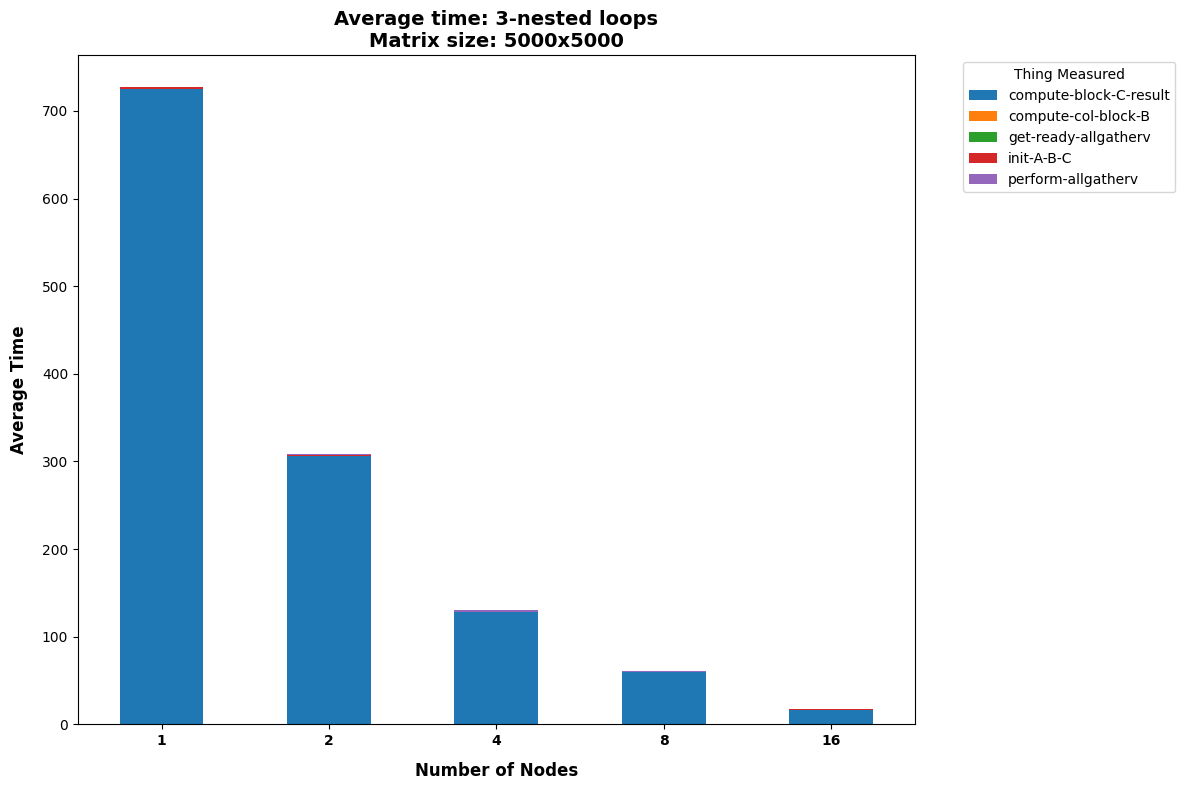
\includegraphics[width=\textwidth]{plots/00-3_nested_loops}
        \caption{Scaling test of the naive implementation}
    \end{figure}

    \begin{figure}
        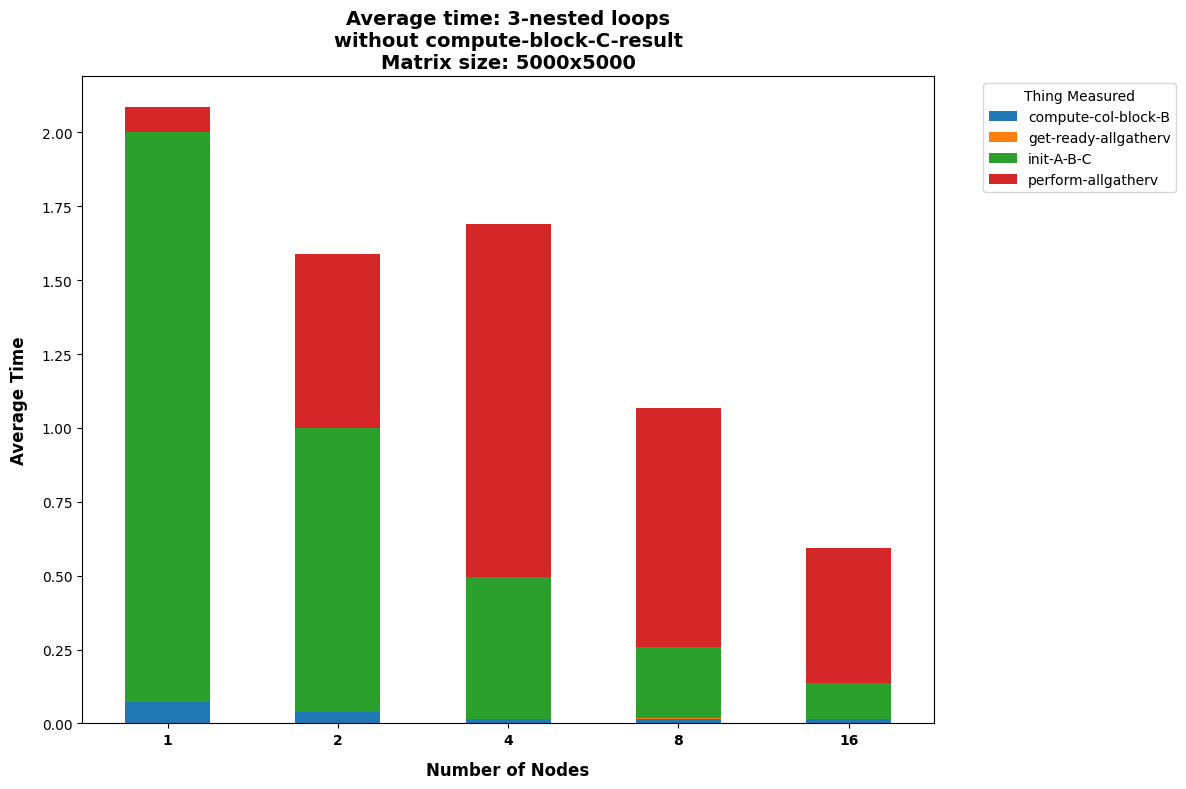
\includegraphics[width=\textwidth]{plots/01-3_nested_loop_no_compute_C_res}
        \caption{Scaling test of the naive implementation: zoom of the time scaling not considering the computation of C time}
    \end{figure}

    \begin{figure}
        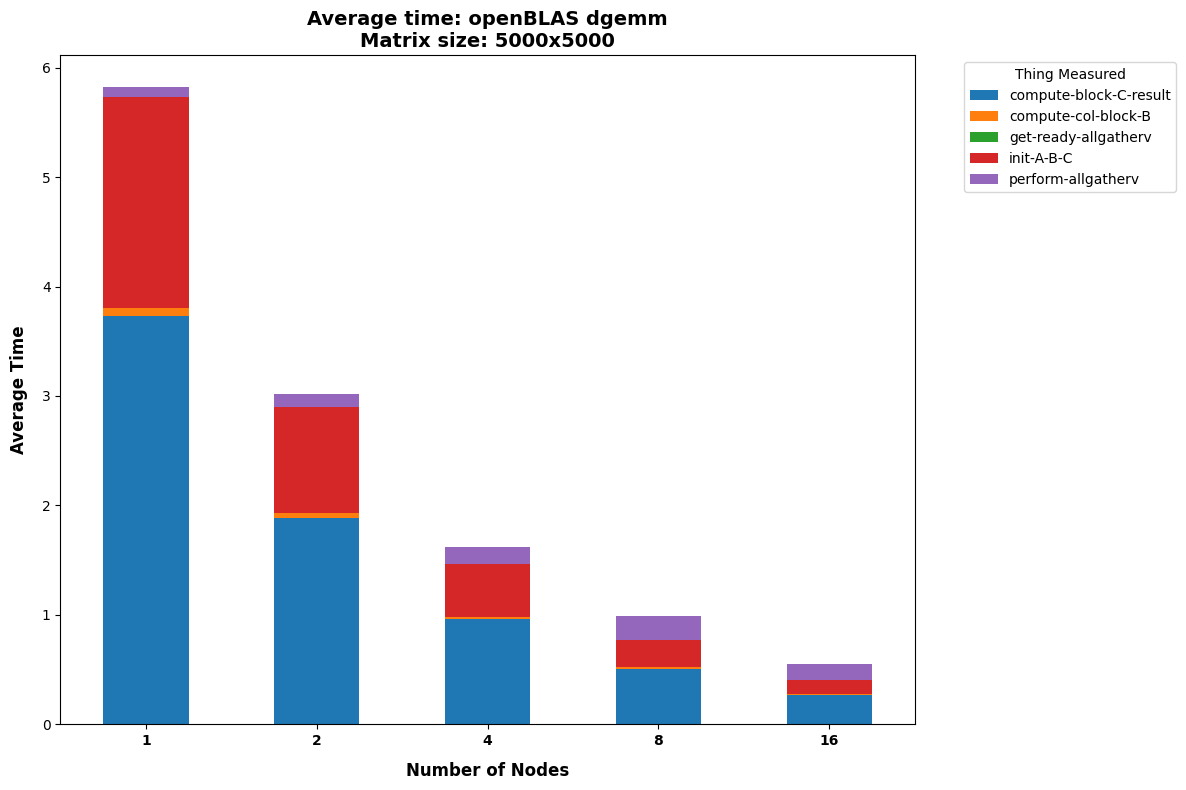
\includegraphics[width=\textwidth]{plots/02-openblas}
        \caption{Scaling test of the BLAS implementation}
    \end{figure}

    \begin{figure}
        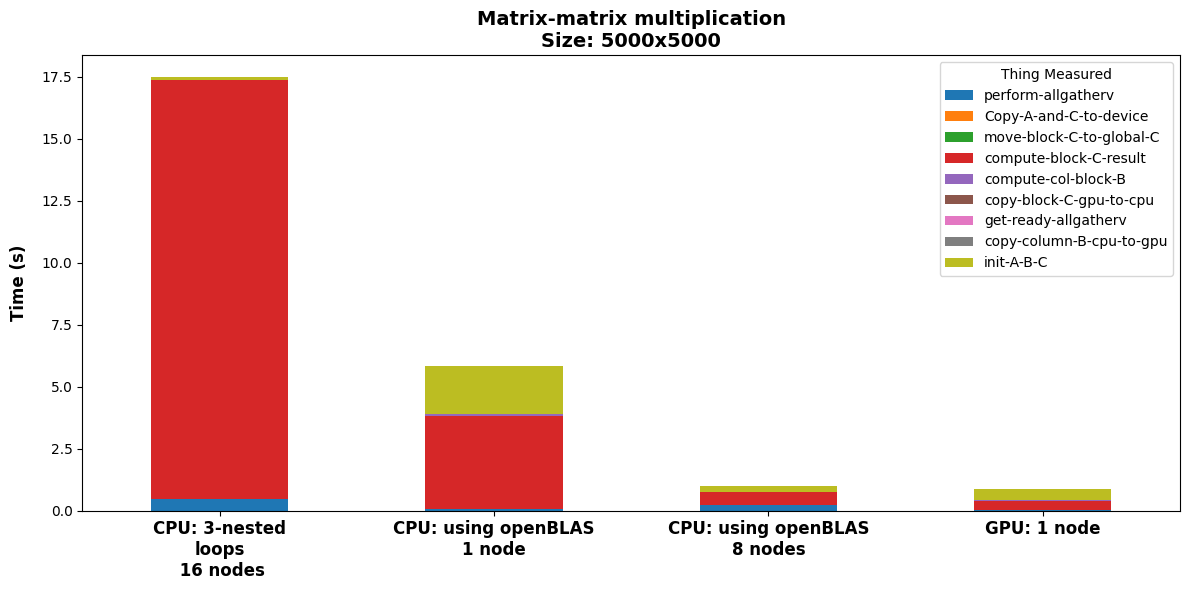
\includegraphics[width=\textwidth]{plots/05-GPU_vs_CPU}
        \caption{Comparison with the same size of matrix between the 3 implementations. This is why the scaling test of the CUDA implementation is done with a bigger matrix}
    \end{figure}

    \begin{figure}
        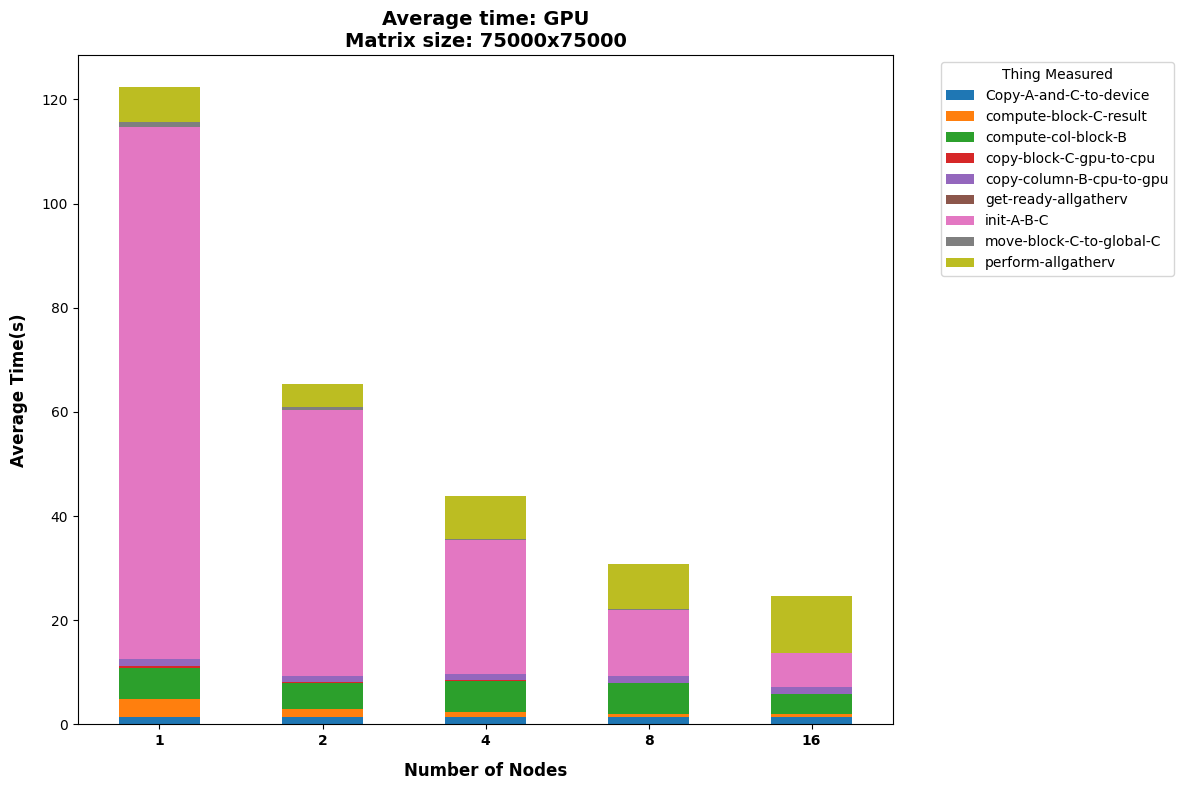
\includegraphics[width=\textwidth]{plots/06_GPU_scaling}
        \caption{Scaling test of the CUDA implementation}
    \end{figure}

\end{document}
